% Fotografía extraída sin modificación del PDF de la familia IND-AX2, p. física 1.
% La foto se identifica como AX2; la tabla del AX4 está en p. física 2.
% Registrar clave bibliográfica indurpack2026indax antes de compilar la integración.
\begin{figure}[H]
    \centering
    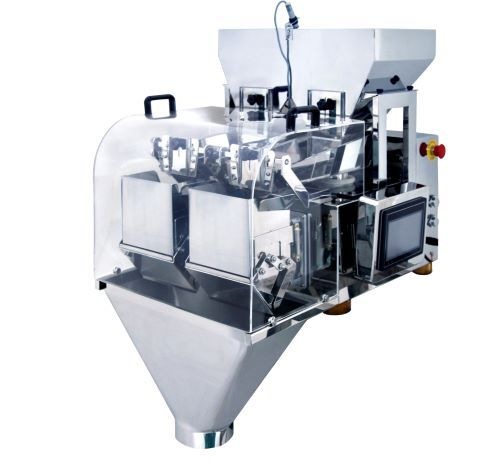
\includegraphics[width=0.48\textwidth]{images/marcopractico/indurpack_indax2_convergencia.jpg}
    \caption{Dosificador IND-AX2 como referente de convergencia de canales hacia una salida común.}
    \label{fig:comercial_convergencia_indax2}
    {\footnotesize Fuente: \textcite{indurpack2026indax}. La fotografía corresponde
    al modelo de dos balanzas; la ficha de la familia incluye la variante IND-AX4
    de cuatro balanzas. La imagen no representa la arquitectura seleccionada
    para San Miguel.}
\end{figure}
